\documentclass{article}
\usepackage{graphicx}
\usepackage[spanish]{babel}
\usepackage[utf8]{inputenc} % Acentos
\usepackage{tikz}
\usepackage{hyperref}
\usepackage[
  top=3cm,
  bottom=3cm,
  left=2cm,
  right=2cm,
  heightrounded,
]{geometry}

\title{Tarea 2}
\author{Martínez Santana Brayan\\
Trad Mateos Kethrim Guadalpe
}

\begin{document}
\maketitle
\section{Definición del problema}
Escribir un programa que pueda aplicar un filtro de color rojo, verde y azul a una imagen y otro filtro especial que pueda generar un mosaico dada una imagen.

\section{Análisis del problema}
\begin{enumerate}
    \item Necesitamos solicitar una imagen a el usuario y que pueda seleccionarla desde su gestor de archivos, para después trabajar con los pixeles de la imagen y poder exponer la imagen modificada sin alterar la imagen original.
    \item La interacción que se tendrá con el usuario tendrá que ser tan amigable como para que el usuario no tenga que escribir la ruta del archivo.
\end{enumerate}
\section{Mejor alternativa} Decidimos utilizar JavaScript por la facilidad que hay para hacer botones en una pagina web y que cualquier navegador puede ejecutar el programa.

\section{Diagrama de flujo} El programa inicia con los botones correspondientes a cargar archivos y aplicar filtros, lo primero que hace el usuario es cargar la imagen, nosotros la posicionamos en la página y accedemos a su arreglo de pixeles con valores rgb, al cual podremos acceder mediante en un método. Posteriormente el usuario podrá escoger un filtro: rojo, azul,verde y mosaico, en caso de que escoga el último se le pedirá que ingrese el número de pixeles que quiere por largo y ancho. El programa termina cuando la imagen se muestra filtrada. El usuario puede usar otros filtros y cargar nuevas imágenes hasta que cierre la página.
	\begin{center}
		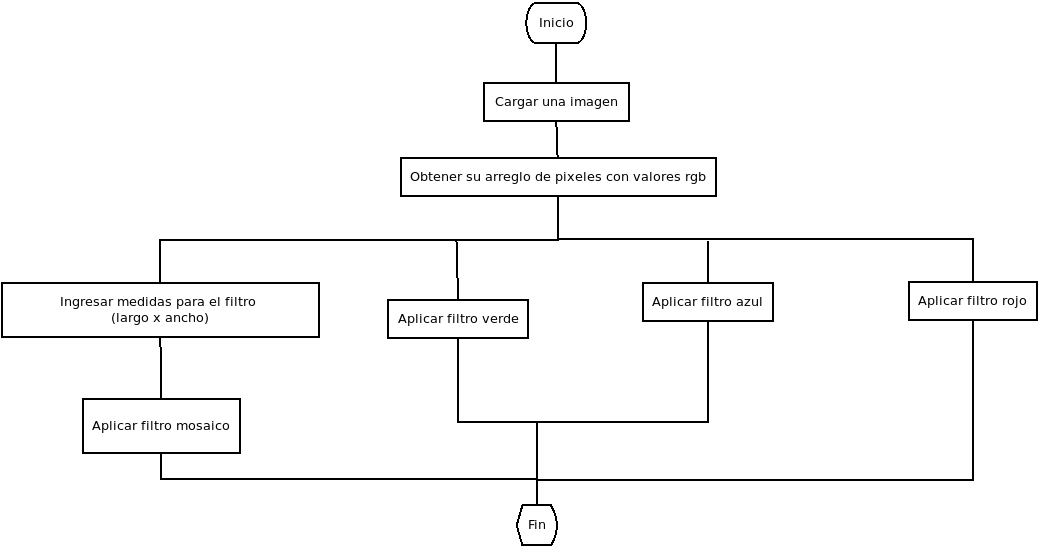
\includegraphics[width=\linewidth]{DiagramaDeFlujo}
	\end{center}

\section{Pensamiento a futuro}
Podemos agregar la opción de que se puedan arrastrar los archivos a la pagina web para trabajar con ellos.\\
También sería muy probable que agreguemos el archivo a una pagina web convencional y que pueda funcionar ahí junto con otros archivos JavaScript.

\section*{Bibliografía}
\begin{enumerate}
    \item \href{https://developer.mozilla.org/es/docs/Web/JavaScript/Referencia/Objetos_globales/Math/random}{Números aleatorios}
    \item\href{https://es.stackoverflow.com/questions/164359/cargar-una-imagen-en-html-y-javascript}{Cargar una imagen en JavaScript}
    \item \href{https://www.anerbarrena.com/javascript-prompt-js-5509/}{Mostrar mensajes en JavaScript}
    \item \href{http://www.etnassoft.com/2016/11/03/manipulacion-de-imagenes-con-javascript-parte-1/?fbclid=IwAR0dXV2vw-8YteOKOKsElT3C-OfrEhC1JJJSqaNuM6Nv6codJGbA1KrKv80}{Manipulación de imágenes en JavaScript}
    \item \href{https://developer.mozilla.org/es/docs/Web/JavaScript/Referencia/Objetos_globales/Error}{Errores en JavaScript}
    \item \href{https://es.stackoverflow.com/questions/56116/cuando-conviene-utilizar-var-let-y-const-en-ecma-script-6}{Var y Let (Diferencias)}
    \item \href{https://developer.mozilla.org/es/docs/Web/JavaScript/Referencia/Objetos_globales/Math/random}{Números random}
    \item \href{https://developer.mozilla.org/es/docs/Web/JavaScript/Referencia/Operadores/Operadores_l\%C3\%B3gicos}{Operadores Lógicos en JavaScript}
    \item \href{https://developer.mozilla.org/es/docs/Web/JavaScript/Referencia/Operadores/instanceof}{Instancias (Operador)}
    \item \href{https://jasmine.github.io/2.0/introduction.html?catch=false}{Jasmine (Ejemplos)}
\end{enumerate}
\end{document}
